\documentclass[paper=a4, fontsize=11pt]{scrartcl}
\usepackage[T1]{fontenc}
\usepackage[utf8]{inputenc}
\usepackage{tikz}
\usepackage{graphicx}
\usepackage{siunitx} 
\usepackage{subcaption}
\usepackage{float}
\usepackage{amsmath}
\usepackage{amsfonts}
\usepackage{enumitem}
\usepackage{cancel}
\usepackage{wrapfig}
\usepackage{imakeidx}
\usepackage{amssymb}
\usepackage{hyperref} 
\usepackage[margin=1in]{geometry}

\makeindex[title=Equations Used]

\title{Math Exam Review: Answers}
\author{Joshua Liu\\
Discord: Josh\#4217} %Got to figure out how to add the tree emojis
\date{\today}

\begin{document}
\maketitle
\section{Introduction}

\section{Exam review questions}
\begin{enumerate}
    \item For what values of the variable(s) is each rational expression not defined?
    \begin{enumerate}
        \item $$\frac{y-2}{5x(y-2)}$$
        
        x and y are not defined, they're variables

        \item $$\frac{x^2-7x+12}{x^2-x-12}$$
        
        x is not defined, it's a variable
    \end{enumerate}
    \item Simplify the following and state restrictions.
    \begin{enumerate}
        \item \begin{align*}
            &\frac{1}{x-1}-\frac{1}{1-x}&x&\neq 1\\
            &=\frac{1}{x-1}+\frac{1}{-(1-x)}&x&\neq 1\\
            &=\frac{1}{x-1}+\frac{1}{x-1}&x&\neq 1\\
            &=\frac{2}{x-1}&x&\neq 1 \\
        \end{align*}
        \item \begin{align*}
            &\frac{a-a^3+\frac{2}{a}}{\frac{8}{a}-2a^3}&a&\neq 0,\frac{8}{a}-2a^3\neq 0\\
            &=\frac{\frac{a^2-a^4+2}{a}}{\frac{8-2a^4}{a}}&a&\neq 0,8-2a^4 \neq 0\\
            &=\frac{a^2-a^4+2}{8-2a^4}&a&\neq 0,a^4\neq 4\\
            &=\frac{(2-a^2)(a^2+1)}{2(4-a^4)}&a&\neq 0,\pm \sqrt{2}\\
            &=\frac{(2-a^2)(a^2+1)}{2(2-a^2)(2+a^2)}&a&\neq 0,\pm \sqrt{2}\\
            &=\frac{a^2+1}{2(2+a^2)}&a&\neq 0,\pm \sqrt{2}\\
            &=\frac{a^2+1}{4+2a^2}&a&\neq 0,\pm \sqrt{2}\\
        \end{align*}
        \item \begin{align*}
            &\frac{x^2+4x-5}{2x^2+11x+5}\div\frac{x^2-3x+2}{2x^2+5x+2}\\
            &=\frac{(x+5)(x-1)}{(2x+1)(x+5)}\div\frac{(x-2)(x-1)}{(2x+1)(x+1)}&x&\neq-\frac{1}{2},-5,-1\\
            &=\frac{(x+5)(x-1)}{(2x+1)(x+5)}\cdot \frac{(2x+1)(x+1)}{(x-2)(x-1)}&x&\neq-\frac{1}{2},-5,-1,2,1\\
            &=\frac{\bcancel{(x+5)}\bcancel{(x-1)}}{\bcancel{(2x+1)}\bcancel{(x+5)}}\cdot \frac{\bcancel{(2x+1)}(x+1)}{(x-2)\bcancel{(x-1)}}&x&\neq-\frac{1}{2},-5,-1,2,1\\
            &=\frac{x+1}{x-2}&x&\neq-\frac{1}{2},-5,-1,2,1\\
        \end{align*}
        \item \begin{align*}
            &\frac{x^2-4x+3}{x^2-x}\\
            &=\frac{(x-3)(x-1)}{x(x-1)}&x&\neq0,1\\
            &=\frac{(x-3)\bcancel{(x-1)}}{x\bcancel{(x-1)}}&x&\neq0,1\\
            &=\frac{x-3}{x}&x&\neq0,1\\
        \end{align*}
        \item \begin{align*}
            &\frac{x^2+x-6}{x^2+5x+4}\div\frac{x^2+4x+3}{x^2+6x+8}\\
            &=\frac{(x+3)(x-2)}{(x+4)(x+1)}\div\frac{(x+3)(x+1)}{(x+4)(x+2)}&x&\neq-4,-1,-2\\
            &=\frac{(x+3)(x-2)}{(x+4)(x+1)}\cdot \frac{(x+4)(x+2)}{(x+3)(x+1)}&x&\neq-4,-1,-2,-3,-1\\
            &=\frac{\bcancel{(x+3)}(x-2)}{\bcancel{(x+4)}(x+1)}\cdot \frac{\bcancel{(x+4)}(x+2)}{\bcancel{(x+3)}(x+1)}&x&\neq-4,-1,-2,-3,-1\\
            &=\frac{(x-2)(x+1)}{(x+1)^2}&x&\neq-4,-1,-2,-3,-1\\
            &=\frac{x^2-x-2}{x^2+2x+1}&x&\neq-4,-1,-2,-3,-1\\
        \end{align*}
        \item \begin{align*}
            &\frac{x-3}{x+2}-\frac{6}{x-4}&x&\neq4,-2\\
            &=\frac{(x-3)(x-4)-6(x+2)}{(x+2)(x-4)}&x&\neq4,-2\\
            &=\frac{x^2-7x+12-6x-12}{(x+2)(x-4)}&x&\neq4,-2\\
            &=\frac{x^2-13x}{(x+2)(x-4)}&x&\neq4,-2\\
            &=\frac{x^2-13x}{x^2-2x-8}&x&\neq4,-2\\
        \end{align*}
        \item \begin{align*}
            &\frac{2x^2-x-1}{3x^2+x-2}\div\frac{2x^2-5x-3}{3x^2-11x+6}\\
            &=\frac{(2x-1)(x+1)}{(3x-2)(x+1)}\div\frac{(2x+1)(x-3)}{(3x-2)(x-3)}&x&\neq\frac{2}{3},-1,3\\
            &=\frac{(2x-1)(x+1)}{(3x-2)(x+1)}\cdot \frac{(3x-2)(x-3)}{(2x+1)(x-3)}&x&\neq\frac{2}{3},-1,3,-\frac{1}{2}\\
            &=\frac{(2x-1)\bcancel{(x+1)}}{\bcancel{(3x-2)}\bcancel{(x+1)}}\cdot \frac{\bcancel{(3x-2)}\bcancel{(x-3)}}{(2x+1)\bcancel{(x-3)}}&x&\neq\frac{2}{3},-1,3,-\frac{1}{2}\\
            &=\frac{2x-1}{2x+1}&x&\neq\frac{2}{3},-1,3,-\frac{1}{2}\\
        \end{align*}
        \item \begin{align*}
            &\frac{3}{x^2-3x-4}-\frac{2}{x^2+5x+4}\\
            &=\frac{3}{(x-4)(x+1)}-\frac{2}{(x+4)(x+1)}&x\neq4,-1,-4\\
            &=\frac{3(x+4)-2(x-4)}{(x-4)(x+1)(x+4)}&x\neq4,-1,-4\\
            &=\frac{3x+12-2x+8}{(x-4)(x+1)(x+4)}&x\neq4,-1,-4\\
            &=\frac{x+20}{(x-4)(x+1)(x+4)}&x\neq4,-1,-4\\
        \end{align*}
    \end{enumerate}
    \item Factor Completely.
    \begin{enumerate}
        \item \begin{align*}
            &4ax^5-\frac{axy^4}{4}\\
            &=ax(4x^4-\frac{y^4}{4})\\
            &=\frac{ax(16x^4-y^4)}{4}\\
            &=\frac{ax(4x^2-y^2)(4x^2+y^2)}{4}\\
            &=\frac{ax(2x-y)(2x+y)(4x^2+y^2)}{4}\\
        \end{align*}
    \end{enumerate}
    \item Solve by factoring
    \begin{enumerate}
        \item \begin{align*}
            2x^2-9x+10&=0\\
            (2x+5)(x+2)&=0\\
            2x+5&=0&-x+2&=0\\
            x&=-\frac{5}{2}&x&=-2\\
            x&=-\frac{5}{2},-2\\
        \end{align*}
        \item \begin{align*}
            2x^2-7x&=4\\
            2x^2-7x-4&=0\\
            (2x+1)(x-4)&=0\\
            2x+1&=0&x-4&=0\\
            x&=-\frac{1}{2}&x&=4\\
            x&=-\frac{1}{2},4\\
        \end{align*}
    \end{enumerate}
    \item Solve $5x^2+1=8x$ using the quadratic formula. Express the answer in simplest radical form.
    \begin{align*}
        5x^2+1&=8x&ax^2+bc+c&=0\\
        5x^2-8x+1&=0&x&=\frac{-b\pm\sqrt{b^2-4ac}}{2a}\\\index{Quadratic Formula!$x=\frac{-b\pm\sqrt{b^2-4ac}}{2a}$}
        x&=\frac{-(-8)\pm\sqrt{(-8)^2-4\cdot 5\cdot 1}}{2\cdot 5}\\
        x&=\frac{8\pm\sqrt{44}}{10}\\
        x&=\frac{8\pm4\sqrt{11}}{10}\\
        x&=\frac{8+4\sqrt{11}}{10}&x&=\frac{8-4\sqrt{11}}{10}\\
        x&=\frac{4+2\sqrt{11}}{5}&x&=\frac{4-2\sqrt{11}}{5}\\
        x&=\frac{4+2\sqrt{11}}{5},\frac{4-2\sqrt{11}}{5}\\
    \end{align*}
    \item Evaluate the expression $E(x)=\frac{x^2+5x+6}{x^2+7x+10}$ for $x=-11$
    \begin{align*}
        E(x)&=\frac{x^2+5x+6}{x^2+7x+10}\\
        E(x)&=\frac{(x+3)(x+2)}{(x+5)(x+2)}\\
        E(x)&=\frac{x+3}{x+2}\\
        E(-11)&=\frac{-11+3}{-11+2}\\
        E(-11)&=\frac{8}{9}\\
    \end{align*}
    \item Solve for x (leave in answers in the radical form if necessary)
    \begin{enumerate}
        \item \begin{align*}
            -2x^2-3x+1&=0\\
            x&=\frac{-(-3)\pm\sqrt{(-3)^2-4\cdot -2\cdot 1}}{2\cdot -2}&x&=\frac{-b\pm\sqrt{b^2-4ac}}{2a}\\
            x&=\frac{3\pm\sqrt{17}}{-4}\\
            x&=\frac{-3\pm\sqrt{17}}{4}\\
            x&=\frac{-3+\sqrt{17}}{4},\frac{-3-\sqrt{17}}{4}\\
        \end{align*}
        \item \begin{align*}
            6^{x-5}&=\frac{1}{36^{2x+5}}\\
            6^{x-5}&=36^{-(2x+5)}\\
            6^{x-5}&=6^{2(-2x-5)}\\
            6^{x-5}&=6^{-4x-10}\\
            x-5&=-4x-10\\
            5x&=-5\\
            x&=-1\\
        \end{align*}
    \end{enumerate}
    \item A rectangular window is continued at the top side with a semi-circle. The perimeter of the window is 10m. Find the dimensions of the window that will maximize the area of the window.
\end{enumerate}
\begin{figure}[h!]
    \centering
    \begin{wrapfigure}{r}{0.5\textwidth}
        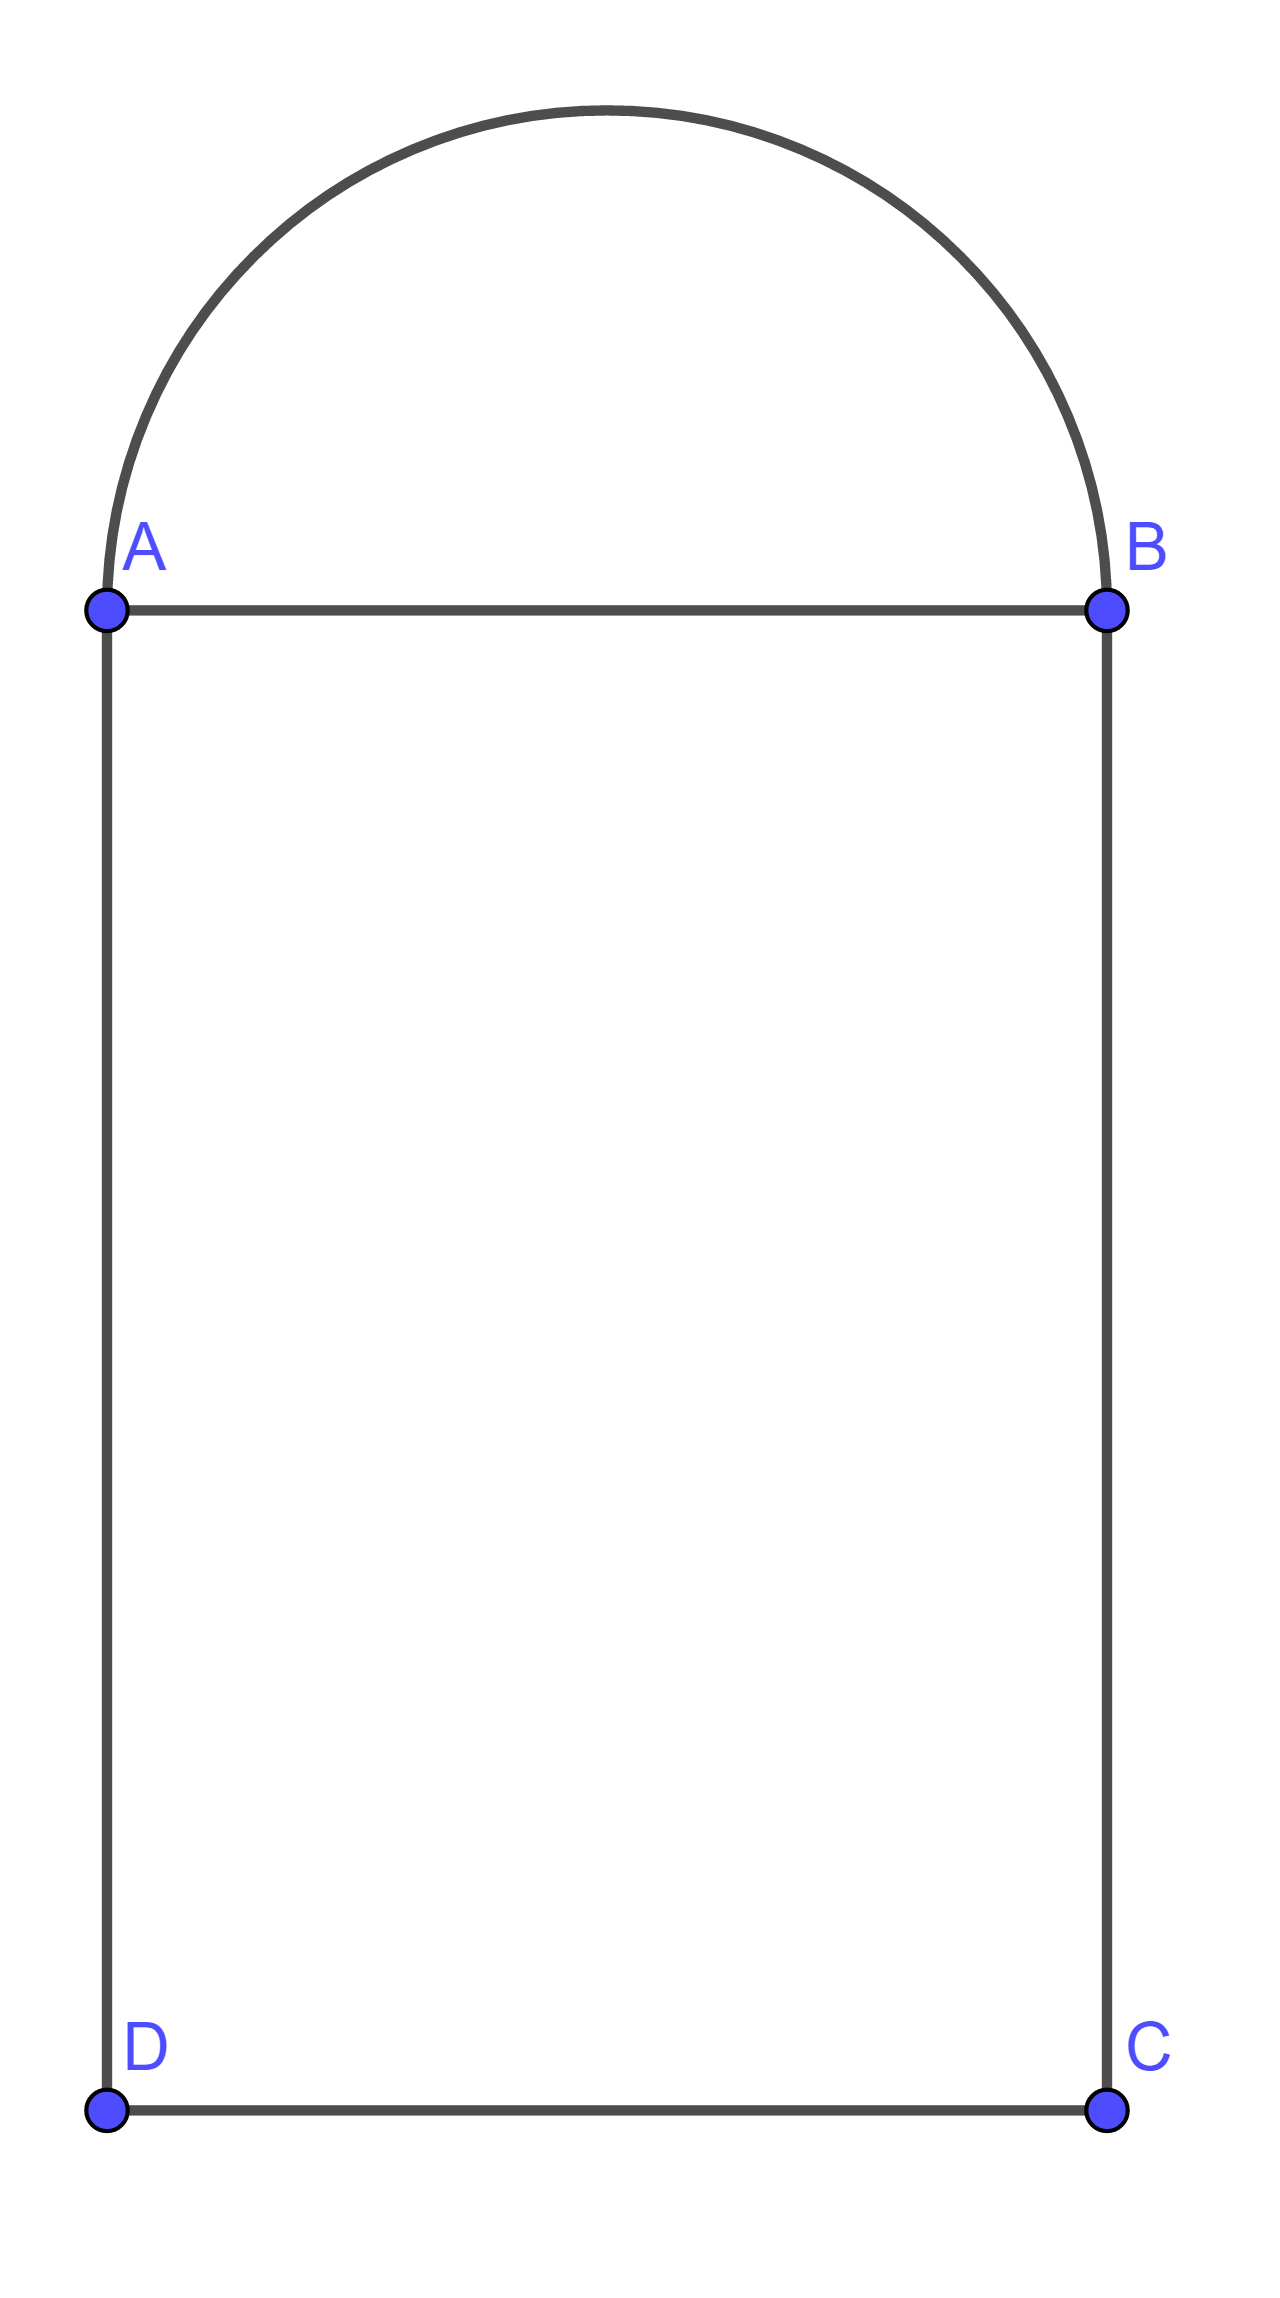
\includegraphics{MathExamReview/8-window.png}
    \end{wrapfigure}    
    \begin{align*}
        2(\overline{AB}+\overline{BC})&=10\\
        \overline{AB}+\overline{BC}&=5\\
        \text{Let x represent }\overline{AB}\\
        Area_{ABCD}&=x(10-x)&Area_{\widehat{AB}}&=(\frac{x}{2})^2\pi\\
        &=10x-x^2&&=\frac{x^2\pi}{4}\\
    \end{align*}
    \begin{align*}
        Area&=10x-x^2+\frac{x^2\pi}{4}\\
        0&=x(10-x+\frac{x\pi}{4})\\
        0&=x(x(\frac{-4+\pi}{4})-10)\\
        x&=0,\frac{40}{\pi-4}\\
    \end{align*}
\end{figure}
Maximum area is the average of the $x_1,x_2$, meaning maximum area is where $x=\frac{20}{\pi-4}$. No need to really worry about this, I was told it doesn't matter.

\begin{enumerate}[resume]
    \item Determine the vertex of $y=-4x^2-16x+5$ and state if it is a maximum or minimum
    
    Remember that looking of the first term (the $-4x^2$) if it's facing up (Is positive), then it is a minimum, if facing down (Is negative), the it is a maximum. In this case, $-4x^2$ is negative, meaning it was a \textbf{maximum}
    \item Complete the square and represent graphically the following quadratic equation $y=-x^2+2x-3$
    
    $$y=-(x^2-2x+3)$$
    $$y=-((x-1)^2+3-1)$$
    $$y=-(x-1)^2-2$$

    Here is the graphical representation, vertex is $(1,-2)$, facing down.

    \begin{figure*}[h!]
        \centering
        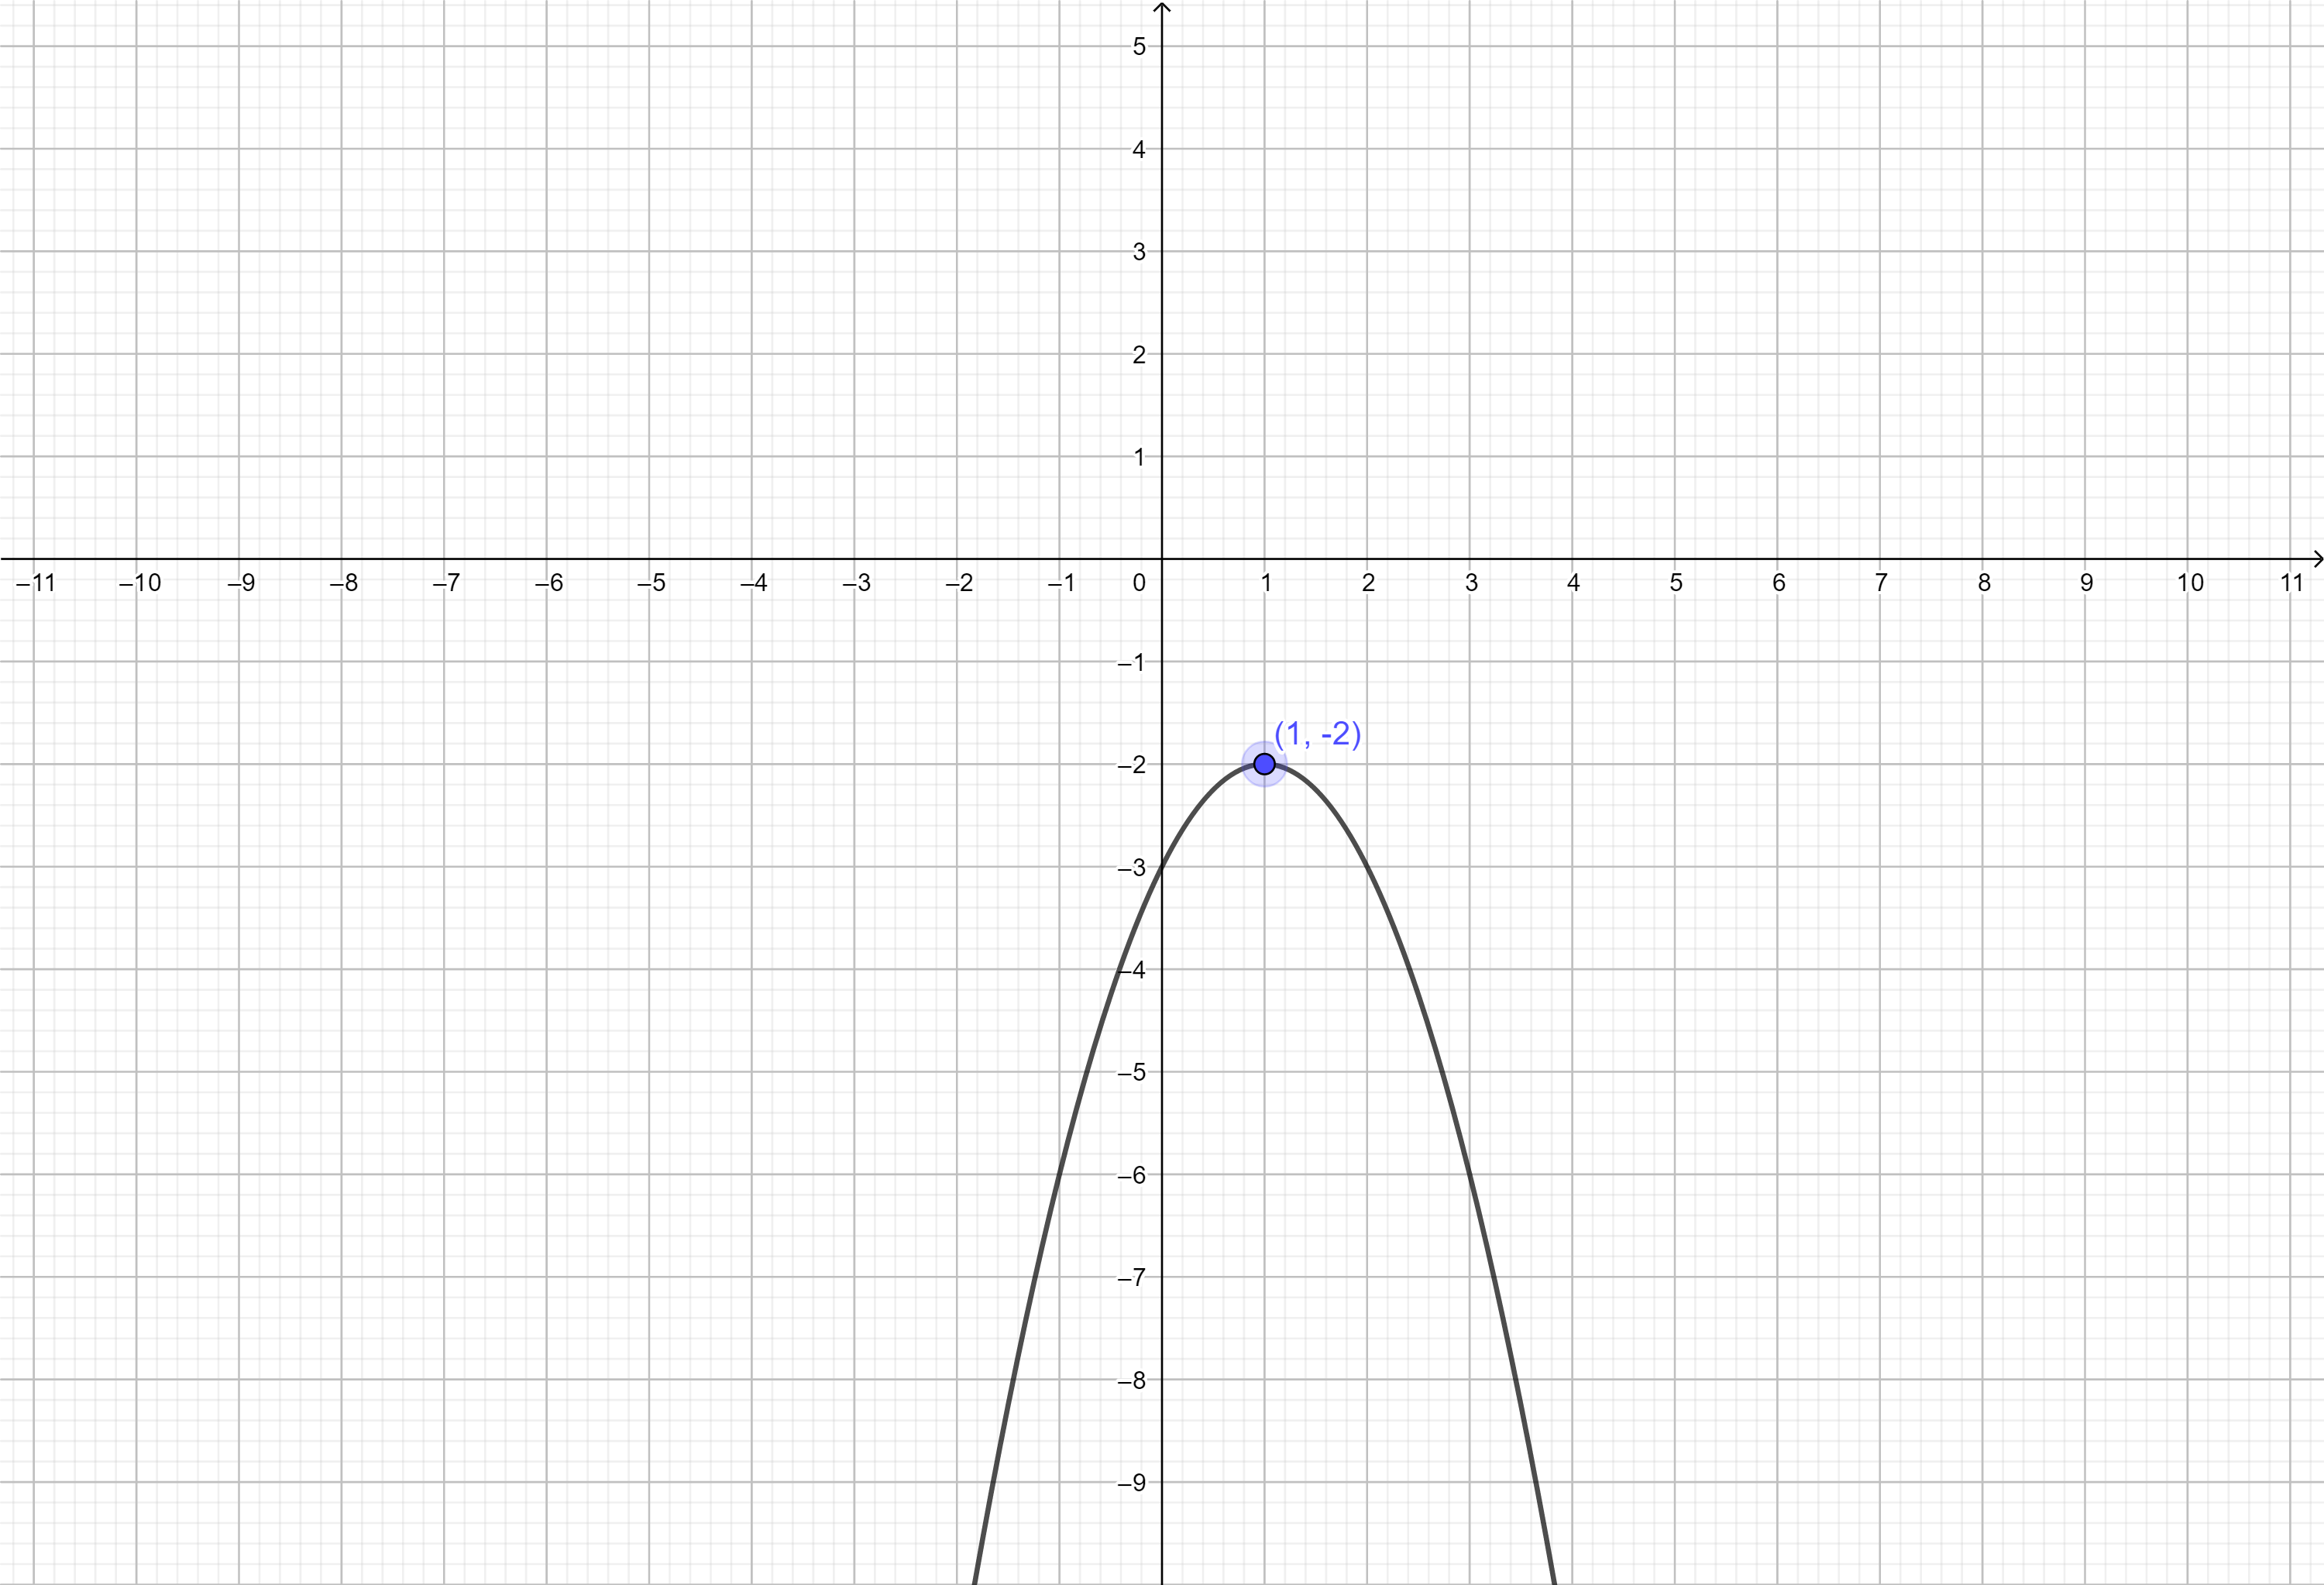
\includegraphics[scale=0.5]{MathExamReview/10-parabola.png}
    \end{figure*}

    \item Given that $\theta$ is an angle in standard position, $0^{\circ}\le\theta\le 360^{\circ}$, with \newline $\cos\theta=-\frac{\sqrt{3}}{2}$. Find all possible values of $\theta$.
    Remember CAST rule 
    \index{CAST Rule!$\sin\theta=\sin\theta$}
    \index{CAST Rule!$\cos\theta=\cos\theta$}
    \index{CAST Rule!$\tan\theta=\tan\theta$}
    \index{CAST Rule!$\sin(180-\theta)=\sin\theta$}
    \index{CAST Rule!$\cos(180-\theta)=-\cos\theta$}
    \index{CAST Rule!$\tan(180-\theta)=-\tan\theta$}
    \index{CAST Rule!$\sin(180+\theta)=-\sin\theta$}
    \index{CAST Rule!$\cos(180+\theta)=-\cos\theta$}
    \index{CAST Rule!$\tan(180+\theta)=\tan\theta$}
    \index{CAST Rule!$\sin(360-\theta)=-\sin\theta$}
    \index{CAST Rule!$\cos(360-\theta)=\cos\theta$}
    \index{CAST Rule!$\tan(360-\theta)=-\tan\theta$}
    \begin{align*}
    \cos\beta&=\frac{\sqrt{3}}{2}\\
    \beta&=30^{\circ}\\
    \end{align*}
    $$\cos(180-\beta)=\cos(180+\beta)=-\cos\beta$$
    \begin{align*}
    180-\beta&=\theta&180+\beta&=\theta\\
    180-30&=\theta&180+30&=\theta\\
    150&=\theta&210&=\theta\\
    \theta&=150^{\circ},210^{\circ}
    \end{align*}
    \item In $\triangle ABC$,$\angle B=107^{\circ}$, $a=18.7$, $c=10.5$. Solve the triangle.
    as you're given two sides and one angle (SAS) you can use the cosine law. $c^2=a^2+b^2-2ab\cos C$ to find the side, the sine law $\frac{\sin A}{a}=\frac{\sin B}{B}=\frac{\sin C}{C}$ to find the angles
    \index{Cosine Law!$c^2=a^2+b^2-2ab\cos C$}
    \index{Sine Law!$\frac{\sin A}{a}=\frac{\sin B}{b}=\frac{\sin C}{c}$}
    \begin{align*}
        b^2&=a^2+c^2-2ac\cos B\\
        b^2&=18.7^2+10.5^2-2\cdot 18.7\cdot 10.5\cdot \cos 107^{\circ}\\
        b&=23.974035297475865\\
        \frac{\sin B}{b}&=\frac{\sin C}{c}\\
        \frac{\sin 107^{\circ}}{23.984}&=\frac{\sin C}{10.5}\\
        0.419&=\sin C\\
        24.8^{\circ}&=\angle C\\
        \angle A &=180-24.8-107\\
        \angle A&=48.2
    \end{align*}
    \item On graph paper provided, sketch one cycle of $y=3\sin \frac{1}{2}(\theta-90^{\circ})-1$
    \begin{align*}
        &\text{Amplitude} = 3\\
        &\text{Equation of the axis}: y=-1\\
        &\text{Phase Shift} = 90^{\circ} right\\
        &\text{Period}: \frac{360}{\frac{1}{2}}=720^{\circ}\\
    \end{align*}
    
    The graph is drawn as shown
    \begin{figure*}[h!]
        \centering
        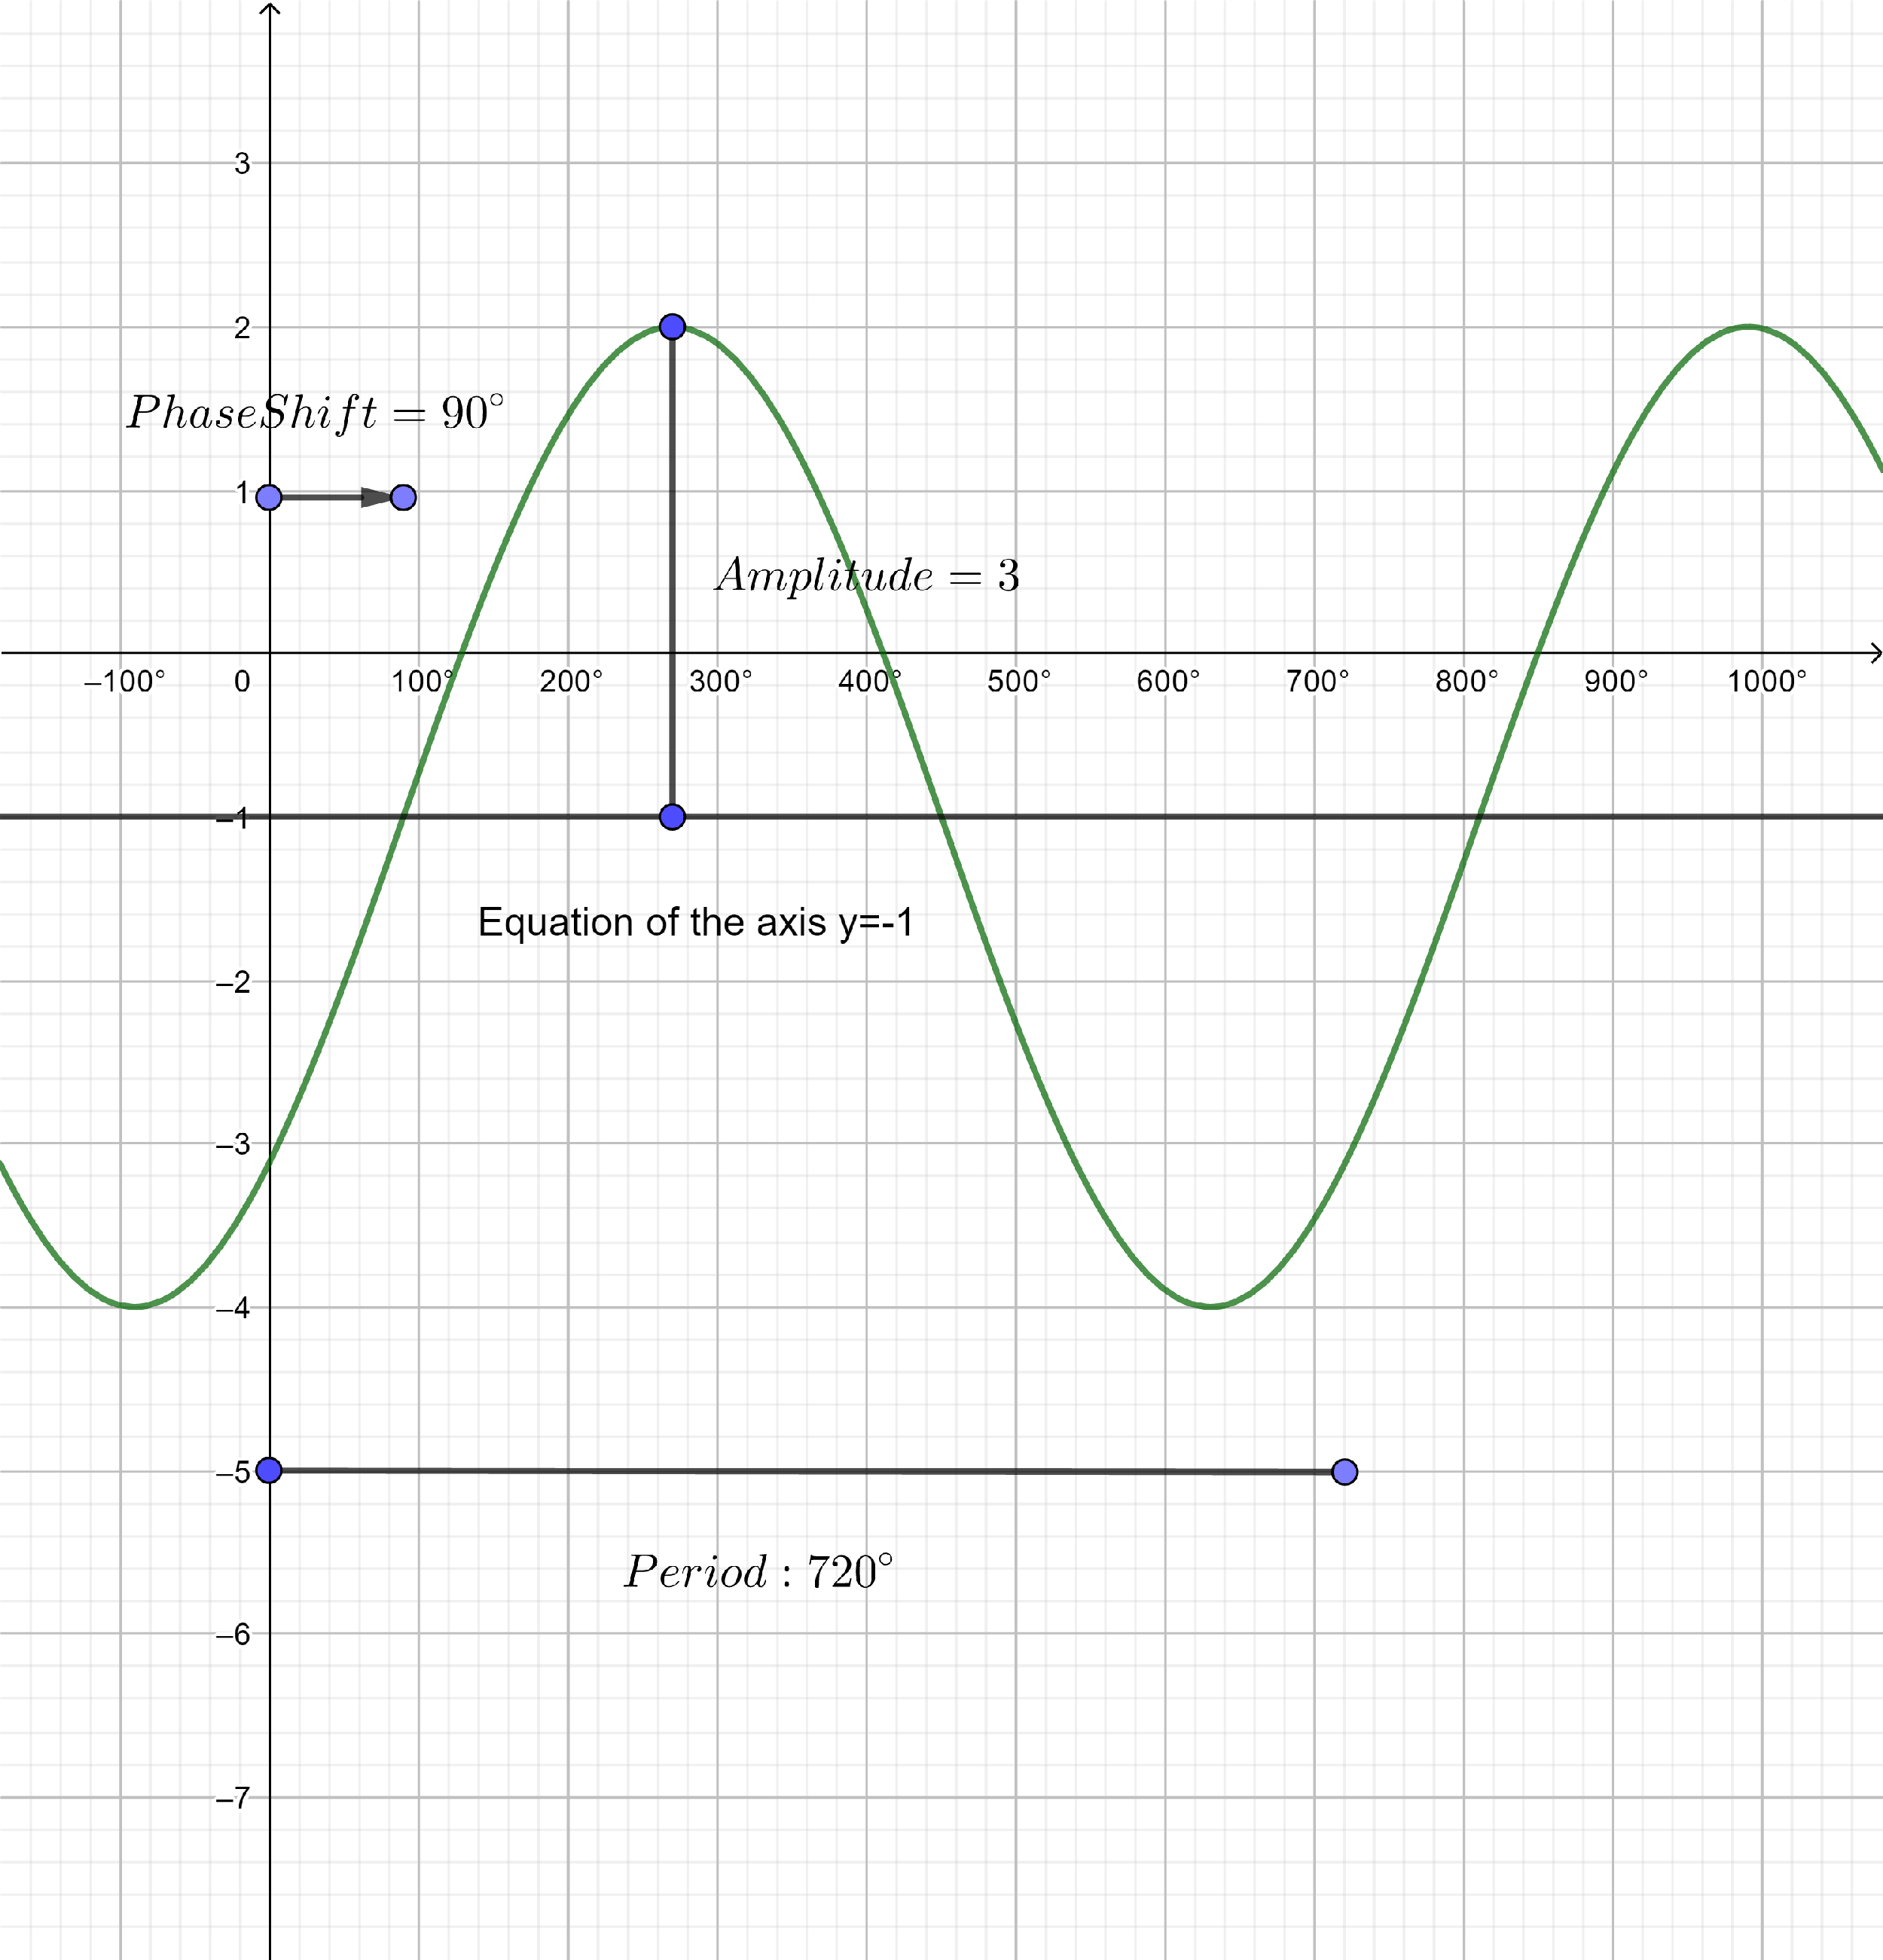
\includegraphics[scale=0.03]{MathExamReview/13-graph1.png}
    \end{figure*}

    \item Given the function $y=-4\cos2(\theta+\frac{180}{3})+5$, state the amplitude, period, phase shift, and range.
    \begin{align*}
        &\text{Amplitude} = 4\\
        &\text{Equation of the axis}: y=5\\
        &\text{Phase Shift} = \frac{180}{3}=60^{\circ} left\\
        &\text{Period}: \frac{360}{2}=180^{\circ}\\
    \end{align*}
    \item Solve the equation for $0\le\theta\le 360^{\circ}$. $\sin\theta(3-4\cos^2\theta)=0$
    \begin{align*}
        \sin\theta&=0&3-4\cos^2\theta&=0\\
        \theta&=0^{\circ},180^{\circ},360^{\circ}&\cos\theta&=-\frac{\sqrt{3}}{2}\\
        \theta&=0^{\circ},180^{\circ},360^{\circ}&\theta&=180-30,180+30\\
        \theta&=0^{\circ},180^{\circ},360^{\circ}&\theta&=150^{\circ},210^{\circ}\\
        \theta&=0^{\circ},150^{\circ},180^{\circ},210^{\circ},360^{\circ}
    \end{align*}
    \item Solve the equation $2\sin^2\theta-\sin\theta-1=0$ for $0\le\theta\le360^{\circ}$.
    \begin{align*}
        \text{Let x represent }\sin\theta\\
        2x^2-x-1&=0\\
        (2x+1)(x-1)&=0\\
        x&=-\frac{1}{2},1\\
        \sin\theta&=-\frac{1}{2}&\sin\theta&=1\\
        \theta&=180+30,360-30&\theta&=90^{\circ}\\
        \theta&=210^{\circ},330^{\circ}&\theta&=90^{\circ}\\
        \theta&=90^{\circ},210^{\circ},330^{\circ}\\
    \end{align*}
    \item Question Missing there's just nothing in the paper
    \item Question Missing there's just nothing in the paper
    \item Prove the identity:
    \begin{enumerate}
        \item $\frac{\sin^2\theta-1}{\cos^2\theta-1}=\frac{1}{\sin^2\theta}-1$
        
        Remember that $\sin^2\theta+\cos^2\theta=1$
        \index{Trig Identity!$\sin^2\theta+\cos^2\theta=1$}
        \begin{align*}
            LS&=\frac{\sin^2\theta-1}{\cos^2\theta-1}&RS&=\frac{1}{\sin^2\theta}-1\\
            &=\frac{-\cos^2\theta}{-\sin^2\theta}&&=\frac{1-\sin^2\theta}{\sin^2\theta}\\
            &=\frac{\cos^2\theta}{\sin^2\theta}&&=\frac{\cos^2\theta}{\sin^2\theta}\\
        \end{align*}
        $$\because LS=RS$$
        $$\therefore \frac{\sin^2\theta-1}{\cos^2\theta-1}=\frac{1}{\sin^2\theta}-1$$
        \item  $\tan\theta+\frac{\cos\theta}{1+\sin\theta}=\frac{1}{\cos\theta}$
        
        Remember that $\tan\theta=\frac{\sin\theta}{\cos\theta}$
        \index{Trig Identity!$\tan\theta=\frac{\sin\theta}{\cos\theta}$}
        \begin{align*}
            LS&=\tan\theta+\frac{\cos\theta}{1+\sin\theta}&RS&=\frac{1}{\cos\theta}\\
            &=\frac{\sin\theta(1+\sin\theta)+\cos\theta}{\cos\theta(1+\sin\theta)}\\
            &=\frac{sin^2\theta+\cos^2\theta+\sin\theta}{\cos\theta(1+\sin\theta)}\\
            &=\frac{1+\sin\theta}{\cos\theta(1+\sin\theta)}\\
            &=\frac{1}{\cos\theta}\\
        \end{align*}
        $$\because LS=RS$$
        $$\therefore \tan\theta+\frac{\cos\theta}{1+\sin\theta}=\frac{1}{\cos\theta}$$
        \item $\frac{\sin x+\tan x}{\cos x+1}=\tan x$
        \begin{align*}
            LS&=\frac{\sin x+\tan x}{\cos x+1}&RS&=\tan x\\
            &=\frac{\sin x+\frac{\sin x}{\cos x}}{\cos x+1}\\
            &=\frac{\frac{\sin x\cos x+\sin x}{\cos x}}{\cos x+1}\\
            &=\frac{\sin x\cos x+\sin x}{\cos x(\cos x+1)}\\
            &=\frac{\sin x(\cos x+1)}{\cos x(\cos +1)}\\
            &=\frac{\sin x}{\cos x}\\
            &=\tan x\\
        \end{align*}
        $$\because LS=RS$$
        $$\therefore \frac{\sin x+\tan x}{\cos x+1}=\tan x$$
    \end{enumerate}
    \item Complete the table
    \begin{center}
        \begin{tabular}{|c|c|c|}
            \hline
            Sine Function&$y=-3\sin(2x-60)+1$&\\
            \hline
            Amplitude&&2\\
            \hline
            Period&&$270^\circ$\\
            \hline
            Phase Shift&&$30^\circ $ left\\
            \hline
            Vertical Shift&&None\\
            \hline
            Domain&&\\
            \hline
            Range&&\\
            \hline
        \end{tabular}
    \end{center}
    \begin{center}
        \begin{tabular}{|c|c|c|}
            \hline
            Sine Function&$y=-3\sin(2x-60)+1$&$\underline{2\sin(\frac{4}{3}(x+30))}$\\
            \hline
            Amplitude&3&2\\
            \hline
            Period&$180^\circ$&$270^\circ$\\
            \hline
            Phase Shift&$30^\circ$ right&$30^\circ $ left\\
            \hline
            Vertical Shift&$1$ up&None\\
            \hline
            Domain&D=\{$x\in\mathbb{R}$\}&D=\{${x\in\mathbb{R}}$\}\\
            \hline
            Range&R=\{$y\in\mathbb{R}\mid -2\le y \le 4$\}&R=\{$y\in\mathbb{R}\mid -2\le y \le 2$\}\\
            \hline
        \end{tabular}
    \end{center}
    \item State a possible equation for the cosine function shown.
    \begin{center}
        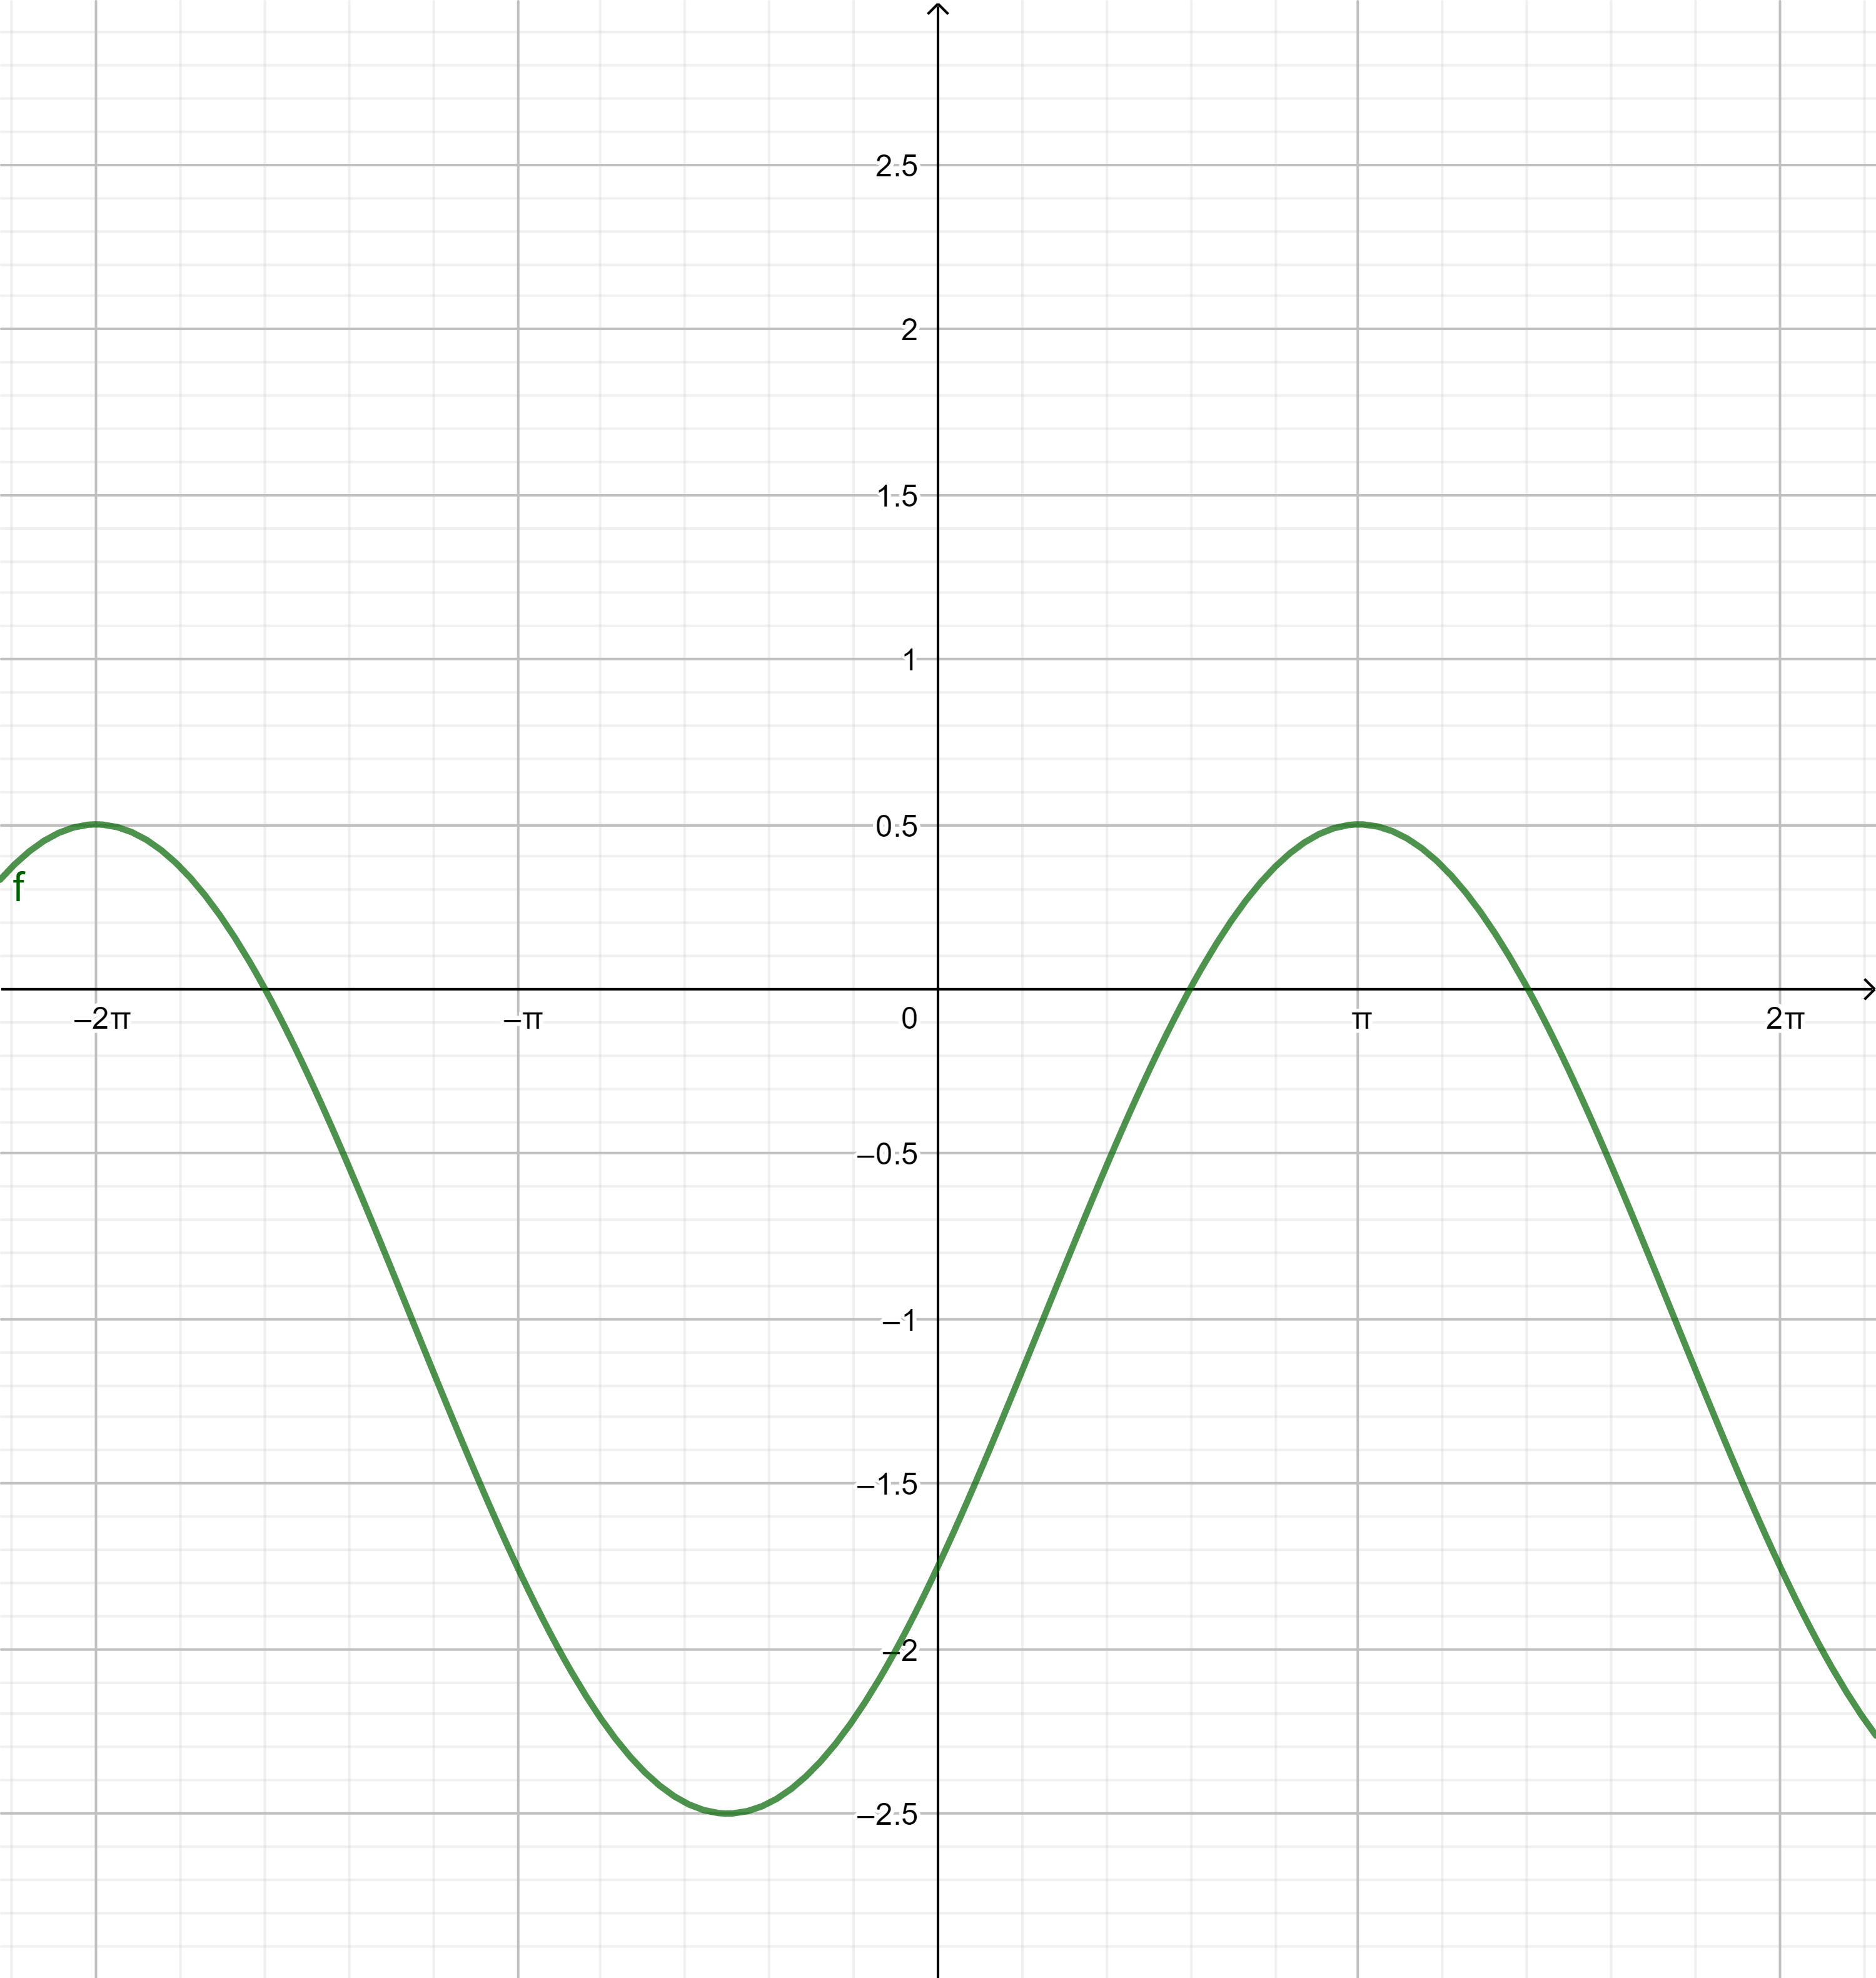
\includegraphics[scale=0.3]{MathExamReview/21-graph.png}
    \end{center}
    \begin{align*}
    Min&=-2.5&Max=0.5\\
    \text{Amplitude}&=\frac{Max-Min}{2}&\text{Period}&=\frac{2\pi}{3\pi}\\
    \text{Amplitude}&=\frac{0.5+2.5}{2}&\text{Period}&=\frac{2}{3}\\
    \text{Amplitude}&=1.5\\
    \text{Equation of the axis: }y&=\frac{Max+Min}{2}&\text{Phase Shift}&=\pi \text{ right}\\
    \text{Equation of the axis: }y&=\frac{-2.5+0.5}{2}\\
    \text{Equation of the axis: }y&=-1\\
    \end{align*}
    \begin{center}
        $$y=1.5\cos(\frac{2}{3}(x-\pi))-1$$
    \end{center}
    \item Consider the function $y=3\sin 2(x+90)+5$.
    
    State the Phase Shift, Period, Vertical displacement, Amplitude, Domain, Range
    \begin{enumerate}
        \item Graph the function over two complete graphs
    \end{enumerate}
    \begin{center}
        \begin{tabular}{|c|c|}
            \hline
            Phase Shift &$90^\circ$ left\\
            \hline
            Period &$\frac{360}{2}=180^\circ$\\
            \hline
            Vertical Displacement &$5$\\
            \hline
            Amplitude &$3$\\
            \hline
            Domain &$D=\{x\in\mathbb{R}\}$\\
            \hline
            Range &$R=\{y\in\mathbb{R}\mid 2\le y \le 8\}$\\
            \hline
        \end{tabular}
    \end{center}
    I will most likely not do the graph, if you really want me to add this, ask me on discord.

    \item Graph the function $y=-3\sin(2x-240)$ for $-180^\circ\le x \le 180^\circ$
    $$y=-3\sin(2x-240)$$
    $$y=-3\sin(2(x-120))$$
    \begin{center}
        \begin{tabular}{|c|c|}
            \hline
            Phase Shift &$120^\circ$ right\\
            \hline
            Period &$\frac{360}{2}=180^\circ$\\
            \hline
            Vertical Displacement &$0$\\
            \hline
            Amplitude &$3$\\
            \hline
            Domain &$D=\{x\in\mathbb{R}\}$\\
            \hline
            Range &$R=\{y\in\mathbb{R}\mid -3\le y \le 3\}$\\
            \hline
        \end{tabular}
    \end{center}
    \begin{center}
        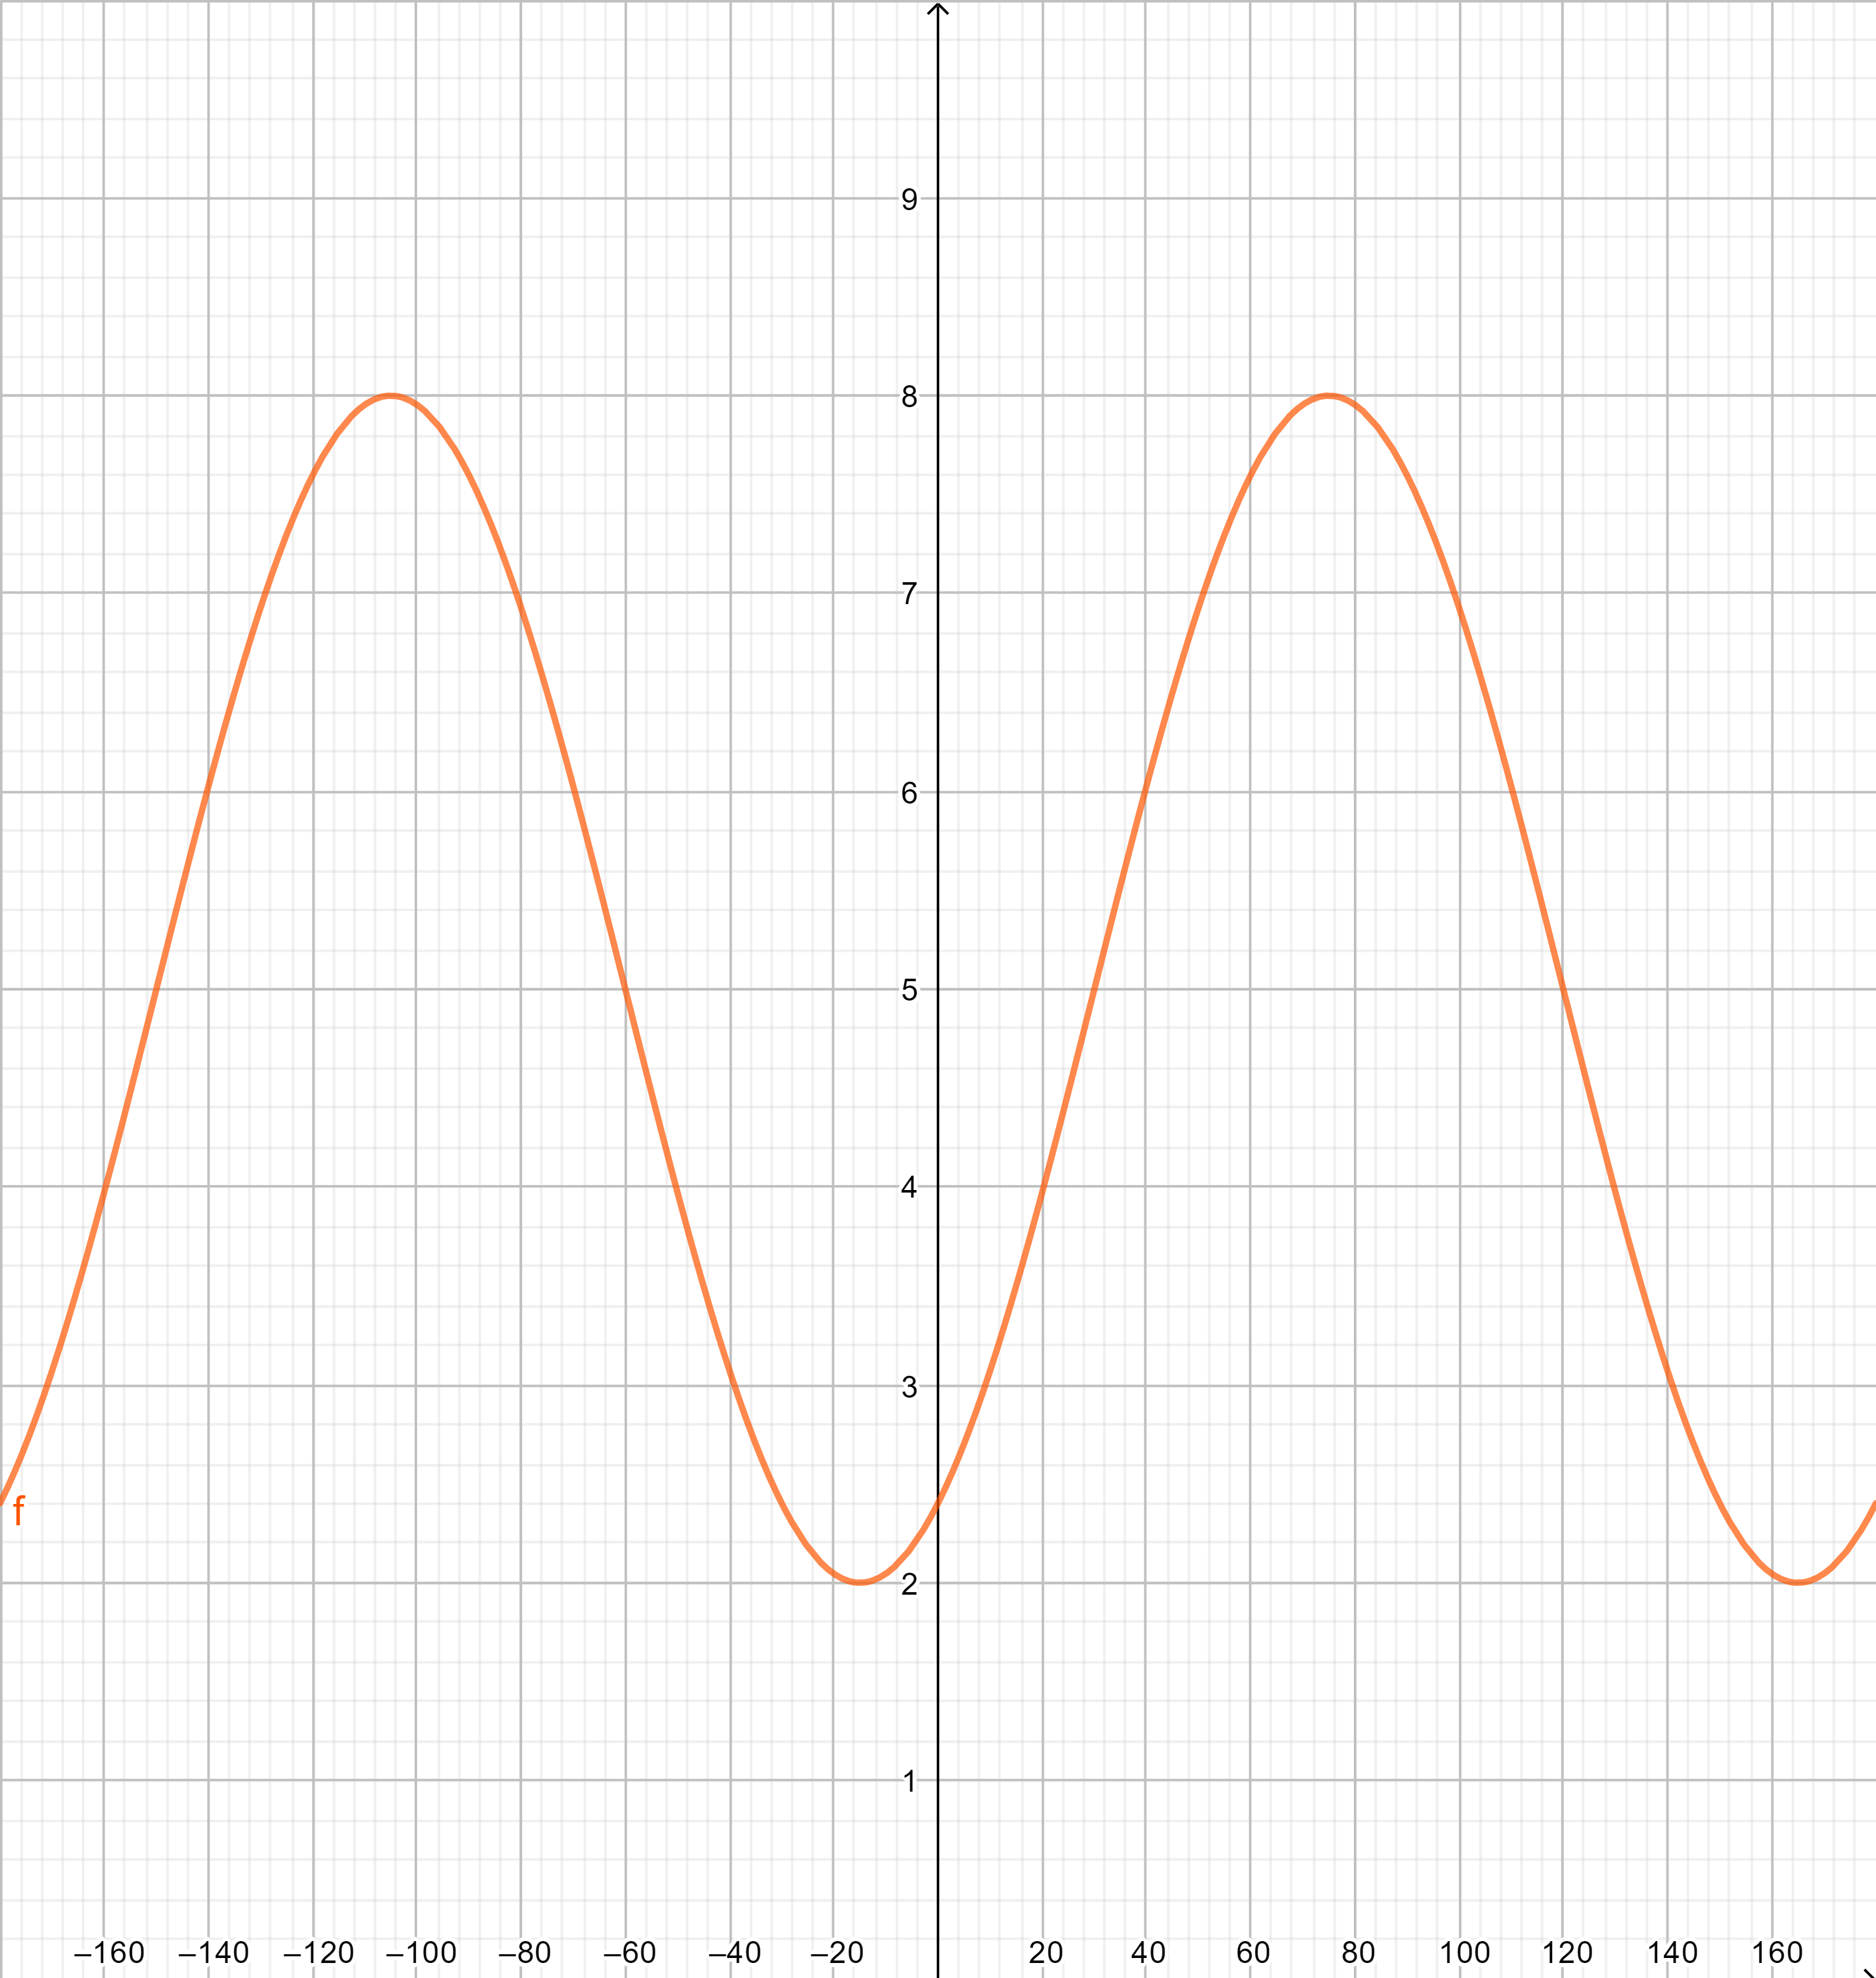
\includegraphics[scale=0.01]{MathExamReview/23-graph.png}
    \end{center}
    \item On a typical day at an ocean port, the water has a maximum depth of $18m$ at 6:00 a.m. The minimum depth of 9 m occurs 6.8 h later. Sketch one complete cycle and write an equation of the form: $h=a\cos b(t-d)+c$ to describe the relationship between the depth $h$ of the water and the time $t$.
    \textit{I'm assuming $t$ is in terms of hours as before it says 6.8 h later}.
    \begin{align*}
        \text{Max}&= 18&\text{Min}&=9\\
        \text{Vertical Displacement}&=\frac{Max+Min}{2}&\text{Amplitude}&=\frac{Max-Min}{2}\\
        \text{Vertical Displacement}&=\frac{18+9}{2}&\text{Amplitude}&=\frac{18-9}{2}\\
        \text{Vertical Displacement/c}&=\frac{27}{2}&\text{Amplitude/a}&=\frac{9}{2}\\
        \text{Phase Shift}&=6.8\text{ right}&\text{Period}&=2*6.8\\
        \text{Phase Shift/d}&=6.8\text{ right}&\text{Period/b}&=13.6\\
        h&=13.5\cos 13.6(t-6.8)+4.5
    \end{align*}
    \begin{center}
        Again, graphs are annoying, if you want me to explain ask me on discord.
    \end{center}
    \item Given the function $f(x)=\frac{x+1}{x^2}$, determine and simplify $f(\frac{1}{x})$
    \begin{align*}
        f(\frac{1}{x})&=\frac{\frac{1}{x}+1}{(\frac{1}{x})^2}\\
        f(\frac{1}{x})&=\frac{\frac{1+x}{x}}{\frac{1}{x^2}}\\
        f(\frac{1}{x})&=\frac{x^2(x+1)}{x}\\
        f(\frac{1}{x})&=x^2+x\\
    \end{align*}
    \item Solve the triangle $\triangle ABC$ in which $AB=23.3cm$ and $BC=26.8cm$ and $\angle ABC=113^\circ$. Round the angles to the nearest degree and lengths to one decimal place. Include diagram.
    
    Use the cosine law to find the missing side$c^2=a^2+b^2-2ab\cos C$. Then use sine law to find the missing angles $\frac{\sin A}{a}=\frac{\sin B}{B}=\frac{\sin C}{C}$.
    \begin{align*}
        c&=23.3&a&=26.8&B&=113^\circ\\
    \end{align*}
    \begin{align*}
        b^2&=a^2+c^2-2\times a\times c\cos B\\
        b^2&=26.8^2+23.3^2-2\times23.3\times26.8\cos 113^\circ\\
        b^2&=1749.11\\
        b&=41.8\\
        \frac{\sin A}{a}&=\frac{\sin B}{B}\\
        \frac{\sin A}{26.8}&=\frac{\sin 113^\circ}{41.8}\\
        \sin A&=\frac{26.8\times\sin 113^\circ}{41.8}\\
        A&=\arcsin(\frac{26.8\times\sin 113^\circ}{41.8})\\
        A&=36^\circ\\
        C&=180-A-B\\
        C&=180-36-113\\
        C&=31^\circ\\
    \end{align*}
    For diagram refer to \href{https://www.triangle-calculator.com/?q=c%3D23.3+a%3D26.8+B%3D113&submit=Solve}{this link}.
    \item Determine how much money is needed today in order to have \$6000 in three years at 6\% compounded quarterly.
    
    Compound interest formula: $A=P(1+\frac{r}{n})^{nt}$. (If you want to understand these variables search online) \index{Compound Interest!$A=P(1+\frac{r}{n})^{nt}$}
    \begin{align*}
        P&=6000&r&=0.06\\
        n&=4&t&=3\\
        A&=6000(1+\frac{0.06}{4})^{3*4}\\
        A&=7173.71\\
    \end{align*}
    \item Suppose you begin a saving program to have \$10 000 after 10 years. You plan to make regular deposits every month into an investment account that pays 6\% compounded monthly, calculate each regular deposit.
    
    This uses the future value annuity formula $FV=P\frac{(1+\frac{r}{n})^{nt}-1}{\frac{r}{n}}$ \index{Future Value Formula!$FV=P\frac{(1+\frac{r}{n})^{nt}-1}{\frac{r}{n}}$}
    \begin{align*}
        n&=12&t&=10\\
        r&=0.06&FV&=10000\\
    \end{align*}
    \begin{align*}
        FV&=P\frac{(1+\frac{r}{n})^{nt}-1}{\frac{r}{n}}\\
        10000&=P\frac{(1+\frac{0.06}{12})^{12\times 10}-1}{\frac{0.06}{12}}\\
        \frac{10000}{\frac{(1+\frac{0.06}{12})^{12\times 10}-1}{\frac{0.06}{12}}}&=P\\
        61.02&=P\\
    \end{align*}
    \item A penny is tossed into the air from a bridge and falls to the water below. The height of the penny $h$ metres, relative to the water $t$ seconds after being thrown is given by $h=-5t^2+10t+20$.
        \begin{enumerate}
            \item Determine the max height of the penny above the water.
            
            I am \textit{pretty }sure that this involves completing the square. \textit{Maybe I got the name wrong}
            \begin{align*}
                h&=-5t^2+10t+20\\
                h&=-5(t^2-2t-4)\\
                h&=-5((t-1)^2-5)\\
                h&=-5(t-1)^2+25
                \text{Vertex: }(1,25)
            \end{align*}
            Maximum height is 25 metres
            \item How long does it take the penny to reach its max height?
            
            it takes 1 second.

            Note: The x value of the maximum is the average of the two x intercepts $\frac{x_1+x_2}{2}$.\index{X value of vertex!$\frac{x_1+x_2}{2}$}
            Replacing $x_1,x_2$ with the quadratic formula you get the x value of vertex is $-\frac{b}{a}$.\index{X value of vertex!$-\frac{b}{2a}$}
        \end{enumerate}
        \item What transformations have been performed on $y=f(x)$ to attain $y=3f(-x+1)-2$?
        
        \begin{center}
            $y=3f(-(x-1))-2$\\ %TODO: Make steps on how to write this
            \text{Vertical stretch by a factor of 3}\\
            \text{Reflect along the y axis}\\
            \text{Horizontal shift 1 unit to the right}\\
            \text{Vertical shift 2 units down}\\
        \end{center}
        \item Describe the transformations applied to $y=\sqrt{49-x^2}$ to produce 
        
        $y=-2\sqrt{49-(x+5)^2}-6$.
        \begin{center}
            \text{Reflect along the x axis}\\
            \text{Vertical stretch by a factor of 2}\\
            \text{Horizontal shift 5 units to the left}\\
            \text{Vertical shift 6 units down}\\
        \end{center}
        \item Given $f(x)=4x^2-5$, determine
        \begin{enumerate}
            \item $f(2)$
            \begin{align*}
                f(2)&=4\times 2^2-5\\
                f(2)&=11\\
            \end{align*}
            \item $f(x)=31$
            \begin{align*}
                31&=4x^2-5\\
                36&=4x^2\\
                x&=\pm 3\\
            \end{align*}
        \end{enumerate}
        \item Determine the inverse of $f(x)=\frac{2}{5+x}-1$, and state its domain.
        \begin{align*}
            f(x)&=\frac{2}{5+x}-1\\
            x&=\frac{2}{5+f'(x)}-1\\
            x+1&=\frac{2}{5+f'(x)}\\
            5+f'(x)&=\frac{2}{x+1}\\
            f'(x)&=\frac{2}{x+1}-5\\
            R&=\{f(x)\in\mathbb{R}\mid f(x)\neq -1\}\\
            D'&=\{x\in\mathbb{R}\mid x\neq -1\}\\
        \end{align*}
        \item For each case,
        \begin{itemize}
            \item find the inverse
            \item state if the inverse is a function or not
        \end{itemize}
        \begin{enumerate}
            \item $f(x)=\frac{1}{2}x-3$
            \begin{align*}
                x&=\frac{1}{2}f'(x)-3\\
                x+3&=\frac{1}{2}f'(x)\\
                f'(x)&=2x+6\\
                &\text{This inverse is a function}
            \end{align*}
            \item $f(x)=x^2+2$
            \begin{align*}
                x&=f'(x)^2+2\\
                x-2&=f'(x)^2\\
                \pm\sqrt{x-2}&=f'(x)\\
                &\text{This inverse is not a function}
            \end{align*}
            \item $f(x)=\frac{2x}{x+1}$
            \begin{align*}
                x&=\frac{2f'(x)}{f'(x)+1}\\
                xf'(x)+x&=2f'(x)\\
                f'(x)(x-2)&=-x\\
                f'(x)&=\frac{x}{2-x}\\
                &\text{This inverse is a function}
            \end{align*}
            \item $f(x)=2(x+2)^2+2$
            \begin{align*}
                x&=2(f'(x)+2)^2+2\\
                x-2&=2(f'(x)+2)^2\\
                \frac{x-2}{2}&=(f'(x)+2)^2\\
                \pm\frac{x-2}{2}-2&=f'(x)\\
                &\text{This inverse is not a function}
            \end{align*}
        \end{enumerate}
    \item Given $f(x)=\frac{1}{x}$ %So desmos is better
    \begin{enumerate}
        \item Sketch the image of $y=2f(-\frac{1}{2}x)+3$
        
        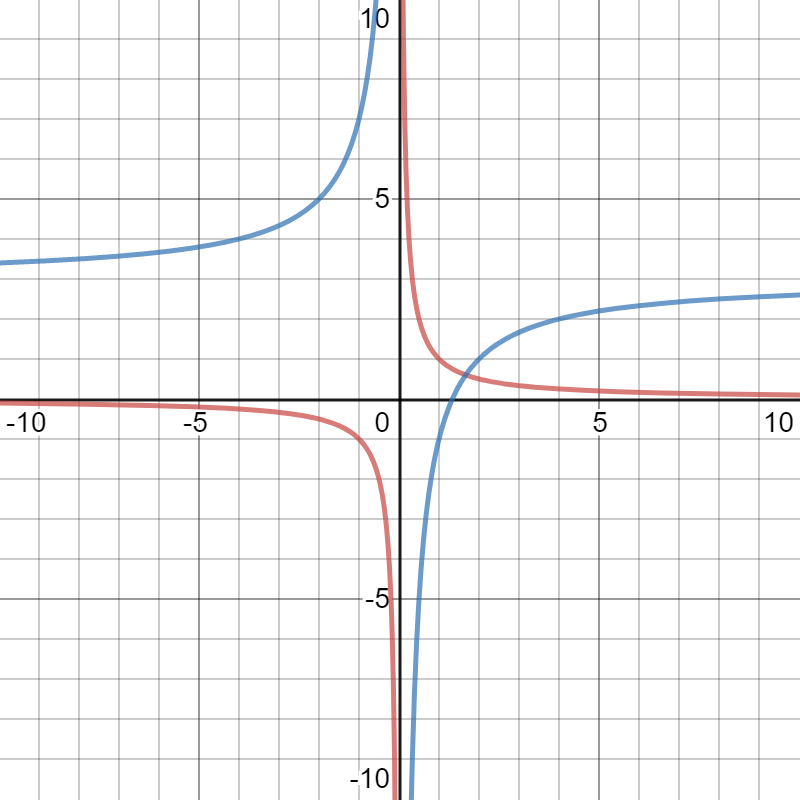
\includegraphics[scale=0.1]{MathExamReview/35-graph.png}

        \item Write and simplify the equation of the image in (a).
        
        \begin{align*}
            y&=2f(-\frac{1}{2}x)+3\\
            y&=2\times\frac{1}{-\frac{1}{2}x}+3\\
            y&=2\times\frac{2}{x}+3\\
            y&=\frac{4}{x}+3\\
        \end{align*}
        \item State the domain and range of the image in (a).
        \begin{align*}
            D&=\{x\in\mathbb{R}\mid x\neq 0\}\\
            R&=\{y\in\mathbb{R}\mid y\neq 3\}\\
        \end{align*}
    \end{enumerate}
\end{enumerate}
\printindex
\end{document}